\newcommand{\nonnegl}{\mathsf{nonnegl}}


\section{Fixed-length MACs}

Previously, we defined what a MAC is, and specified correctness and security definitions for MACs. In this section, we'll define a fixed-length MAC for length $\ell(n)$.

\begin{theorem}
    If $F : \{0, 1\}^n \to \{0, 1\}^n$ is a PRF, then $\Pi = (\mathsf{Gen}, \mathsf{Mac}, \mathsf{Verify})$ (constructed below) is a MAC, as defined with EF-CMA security.

    \begin{algorithmic}[1]
        \Function{Gen}{$1^n$}
            \State \Return $k \in \{0, 1\}^n$
        \EndFunction
        \Statex
        \Function{Mac}{$k$, $m$}
            \State \Return $F_k(m)$
        \EndFunction
        \Statex
        \Function{Verify}{$k$, $m$, $t$}
            \State \Return $t \overset{?}{=} F_k(m)$
        \EndFunction
    \end{algorithmic}

    That is, we just compute the PRF on our message as the MAC.
\end{theorem}

\begin{proof}
    To prove security, suppose for contradiction that there exists an adversary $A$ that breaks the security for $\Pi$. We'd like to construct an adversary $B$ that breaks the security of the PRF.

    Here, the adversary $A$ expects queries for tags, given messages as input. $B$ can simply forward these requests on to $F$, and return the response back to $A$. Further, $A$ outputs a pair $(m^*, t^*)$, which $B$ can send $m^*$ to $F$, and output whether $t = t^*$.

    \begin{center}
        \begin{tikzpicture}
            \draw (3, 0) rectangle (8, 5.5);
            \draw (5, 0.5) rectangle (7.5, 5);
            \node at (3.25, 5.25) {$B$};
            \node at (5.25, 4.75) {$A$};

            \draw (5.5, 4) edge[->] node[right, pos=0] {$m$} (2.5, 4)
                (2.5, 3.5) edge[->] node[right, pos=1] {$t$} (5.5, 3.5);
            \node[left] at (2.5, 3.75) {$F_k$};
            \node at (5.5, 3.1) {$\vdots$};
            \node at (4.5, 3.1) {$\vdots$};
            \draw (5.5, 2.5) edge[->] node[right, pos=0] {$(m^*, t^*)$} (4.5, 2.5);

            \draw (3.5, 2.5) edge[->] node[right, pos=0] {$m^*$} (2.5, 2.5);
            \node[left] at (2.5, 2.25) {$F_k$};
            \draw (2.5, 2) edge[->] node[right, pos=1] {$t$} (3.5, 2);
            \draw (3.5, 1) edge[->] node[right, pos=0] {$t \overset{?}{=} t^*$} (2.5, 1);
        \end{tikzpicture}
    \end{center}

    Analyzing the probability for $B$, we have
    \[
        \abs{\Pr(B^{F_k(\cdot)}(1^n) = 1) - \Pr(B^{R_n(\cdot)}(1^n) = 1)}
        = \abs{\varepsilon_A(n) - \frac{1}{2^n}}
        = \nonnegl(n)
    .\]
    Here, the first term is because the correctness follows immediately from the correctness of $A$, and the second term is due to the fact that the output of $R_n$ is random.
\end{proof}

\section{Variable-length MACs}

Now, let us look at messages with lengths that are a multiple of $n$. In particular, we have a few blocks $m_1, \ldots, m_{\ell}$, each of size $n$. There are a few ways to do this, but we'll look at a method similar to the counter mode we looked at last time.

\begin{center}
    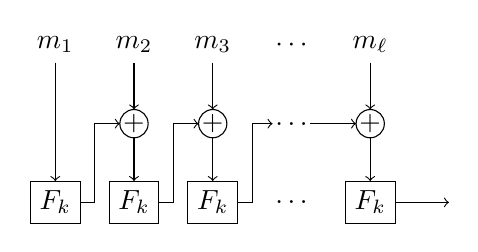
\begin{tikzpicture}
        \node (m1) at (0, 2) {$m_1$};
        \node (m2) at (1, 2) {$m_2$};
        \node (m3) at (2, 2) {$m_3$};
        \node (mdots) at (3, 2) {$\cdots$};
        \node (ml) at (4, 2) {$m_{\ell}$};

        \node[draw] (fk1) at (0, 0) {$F_k$};
        \node[draw] (fk2) at (1, 0) {$F_k$};
        \node[draw] (fk3) at (2, 0) {$F_k$};
        \node at (3, 0) {$\ldots$};
        \node[draw] (fkl) at (4, 0) {$F_k$};

        \node[outer sep=0pt, inner sep=0pt, draw, circle] (fk1+m2) at (1, 1) {$+$};
        \node[outer sep=0pt, inner sep=0pt, draw, circle] (fk2+m3) at (2, 1) {$+$};
        \node[outer sep=0pt, inner sep=1pt] (xor-dots) at (3, 1) {$\ldots$};
        \node[outer sep=0pt, inner sep=0pt, draw, circle] (dots+ml) at (4, 1) {$+$};

        \draw (m1) edge[->] (fk1)
            (m2) edge[->] (fk1+m2)
            (m3) edge[->] (fk2+m3)
            (ml) edge[->] (dots+ml);

        \draw[->] (fk1) -- ++(0.5, 0) |- (fk1+m2);
        \draw[->] (fk2) -- ++(0.5, 0) |- (fk2+m3);
        \draw[->] (fk3) -- ++(0.5, 0) |- (xor-dots);

        \draw[->] (xor-dots) -- (dots+ml);
        \draw (fk1+m2) edge[->] (fk2)
            (fk2+m3) edge[->] (fk3)
            (dots+ml) edge[->] (fkl);
        \draw (fkl) edge[->] ++(1, 0);
    \end{tikzpicture}
\end{center}

This construction avoids having to store a tag equal in length to the message, but this is not secure, due to length extension attacks. In particular, suppose we query for the tag $t$ associated with $0^n$. We can then query another tag $t'$ for $0^n \oplus t$. Observe here that $t'$ is also the tag for $0^{2n}$.

A solution is to use different keys for each PRF, but this isn't too efficient, since we're still calling the PRF once per block of length $n$. We'll instead improve this to use only one block cipher call---we do some preprocessing and only call $F_k$ once on the output of the preprocessing.

In particular, we'll claim that applying a universal hash function to the input and then applying the block cipher is a secure MAC.

\begin{definition}[Universal Hash Function]
    A function $h : \mathcal{F} \times \mathcal{F}^* \to \mathcal{F}$ (where $\mathcal{F}$ is a field of size $2^m$) is a universal hash function if for all $m, m' \in \mathcal{F}^{\le \ell}$ (i.e. $m$ and $m'$ have length at most $\ell$),
    \[
        \Pr_s(h(s, m) = h(s, m')) \le \frac{\ell}{\abs{F}}
    .\]
    That is, the probability of collision is small.
\end{definition}

Crucially here, we fix $m$ and $m'$, and we sample $s$. (If we fix an $s$, we can almost surely find an $m$ and $m'$ that collide.)

Today, we'll look at the following function:
\[
    h(s, m_0, \ldots, m_{\ell - 1}) = m_0 + m_1 s + m_2 s^2 + \cdots + m_{\ell - 1} s^{\ell - 1} + s^{\ell}
.\]

\begin{claim}
    The function defined by
    \[
        h(s, m_0, \ldots, m_{\ell - 1}) = m_0 + m_1 s + m_2 s^2 + \cdots + m_{\ell - 1} s^{\ell - 1} + s^{\ell}
    \]
    is a universal hash function.
\end{claim}

\begin{proof}
    We'd like to argue that for a fixed $m$ and $m'$, and a random $s$, the probability that there is a collision is at most $\frac{\ell}{\abs{\mathcal{F}}}$.

    We'll look at
    \[
        h(x, m_0, \ldots, m_t) - h(x, m_0', \ldots, m_t') = (m_0 - m_0') + \cdots + (m_{t - 1} - m_{t-1}') x^{\ell - 1}
    .\]
    If there is a collision, this difference is 0. The probability that this polynomial of degree at most $\ell$ has a zero at $x$ is at most $\frac{\ell}{\abs{\mathcal{F}}}$, since it has at most $\ell$ zeroes. This means that $h$ is indeed a universal hash function.
\end{proof}

\begin{claim}
    The MAC given by $F_k(h(s, m_1, \ldots, m_{\ell}))$, for the universal hash function $h$ given prior, is secure. (This is a slight variation on the Carter--Wegman MAC.)
\end{claim}

\begin{proof}
    Suppose for contradiction that there exists a nu-PPT $A$ that breaks the security of this scheme.

    Here, for appropriately generated $k$ and $s$, $A$ makes queries $m \mapsto F_k(h_s(m))$, and outputs $(m^*, t^*)$.

    We'd like to create an adversary $B$ that either breaks the security of the PRF, or breaks the security of the universal hash function.

    $B$ will start by sampling $s \in \mathcal{F}$. When given the query for $m_1$, it computes $h_s(m_1)$ and queries for $F_k(h_s(m_1))$, which it sends back to $A$. If $F_k$ was actually pseudorandom, then $A$ is given a pseudorandom input, and if $F_k$ was random $R_n$, then $A$ is given a random input.

    $A$ must still be able to generate pairs $(m^*, t^*)$ even when given a random input, due to the security of the PRF.

    \begin{center}
        \begin{tikzpicture}
            \draw (2, 0) rectangle (8, 5.5);
            \draw (5, 0.5) rectangle (7.5, 5);
            \node at (2.25, 5.25) {$B$};
            \node at (5.25, 4.75) {$A$};

            \node at (3.5, 4.5) {sample $s \in \mathcal{F}$};

            \node (hsm) at (3.5, 4) {$h_s(m)$};
            \draw (5.5, 4) edge[->] node[right, pos=0] {$m$} (hsm)
                (hsm) edge[->] (1.5, 4)
                (1.5, 3.5) edge[->] node[right, pos=1] {$t$} (5.5, 3.5);
            \node[left] at (1.5, 3.75) {$F_k$};
            \node at (5.5, 3.1) {$\vdots$};
            \node at (4.5, 3.1) {$\vdots$};

            \node (hash-m-star) at (3.5, 2.5) {$h_s(m^*)$};
            \draw (5.5, 2.5) edge[->] node[right, pos=0] {$(m^*, t^*)$} (hash-m-star)
                (hash-m-star) edge[->] (1.5, 2.5);
            \node[left] at (1.5, 2.25) {$F_k$};
            \draw (1.5, 2) edge[->] node[right, pos=1] {$t$} (3.5, 2);
            \draw (3.5, 1) edge[->] node[right, pos=0] {$t \overset{?}{=} t^*$} (1.5, 1);
        \end{tikzpicture}
    \end{center}

    Let $E$ be the event that there exists an $m, m' \in L \cup \{m^*\}$, such that $h_s(m) = h(m')$. If $E$ does not happen, then the hash function never collides. This means that the attacker only sees random values depending on distinct inputs, so this reduces to the case from earlier (when the MAC is just $F_k$).

    As such, we'd like to show that collisions in $h_s(\cdot)$ occur with negligible probability.

    To show this, suppose for contradiction that collisions actually do occur with non-negligible probability. We then want to construct an adversary $B$ utilizing $A$ that just outputs $m$ and $m'$ such that when $s$ is sampled, $h_s(m) = h_s(m')$ with high probability.

    $B$ will pick a random $i, j \in \{1, \ldots, q+1\}$ (here suppose $i < j$), where $q$ is the number of MAC queries. We then run $A$ until the $j$th query. Taking the $i$th and $j$th query, we then output $m_i$ and $m_j$ as our pair of messages. We still need to entertain the queries made by $A$, so we can just return random values for tags (giving the same value if it requests it for the same message).

    \begin{center}
        \begin{tikzpicture}
            \draw (2, 0) rectangle (8, 6);
            \draw (5, 0.5) rectangle (7.5, 5.5);
            \node at (2.25, 5.75) {$B$};
            \node at (5.25, 5.25) {$A$};

            \node[align=center] at (3.5, 5) {\small $i, j \xleftarrow{\$} \{1, \ldots, q+1\}$};

            \draw (5.5, 4) edge[->] node[right, pos=0] {$m_1$} (4.5, 4)
                (4.5, 3.5) edge[->] node[left, pos=0] {sample $t_1$} node[right, pos=1] {$t_1$} (5.5, 3.5);
            \node at (5.5, 3.1) {$\vdots$};
            \node at (4.5, 3.1) {$\vdots$};

            \draw (5.5, 2.5) edge[->] node[right, pos=0] {$m_i$} (4.5, 2.5)
                (4.5, 2) edge[->] node[left, pos=0] {sample $t_i$} node[right, pos=1] {$t_i$} (5.5, 2);
            \node at (5.5, 1.6) {$\vdots$};
            \node at (4.5, 1.6) {$\vdots$};

            \draw (5.5, 1) edge[->] node[right, pos=0] {$m_j$} (4.5, 1);

            \draw (3, 0.5) edge[->] node[right, pos=0] {$(m_i, m_j)$} (1.5, 0.5);
        \end{tikzpicture}
    \end{center}

    By assumption, we know that $E$ occurs with non-negligible probability. That is, among the queries made by $A$, there is a non-negligible probability that $h_s(m_i) = h_s(m_j)$. Since here the implementation of $B$ just picks out a pair of random queries from those made by $A$, the pair $(m_i, m_j)$ output by $B$ also has a collision with non-negligible probability. (In particular, with probability $\Pr(E) / q^2$.

    This breaks the definition of a universal hash function, which is a contradiction.
\end{proof}

So far, we know how to generate tags of fixed length, and of lengths that are a multiple of $n$. If we have a message that is not a multiple of $n$, we could potentially just pad the input with 0's, but this causes an issue, as $m$ and $m \concat 0$ have the same tag.

Instead, one solution is to put the size of the message in the first block, and we can still put the padding at the end. This way, if the messages differ by length, the first block will be different, and if the messages do not differ by length, then we're essentially just ignoring the padding. This gives us a MAC for arbitrary-length messages.

\section{Authenticated Encryption Schemes}

We've talked about confidentiality and integrity separately, but generally we want both properties---when Alice sends a message to Bob, we'd like for any eavesdropper to be unable to recover the message, \emph{and} we'd like Bob to be able to verify that the message actually came from Alice.

A scheme that achieves both of these conditions is called an \emph{authenticated encryption scheme}.

\begin{definition}[Authenticated Encryption Scheme]
    A scheme $\Pi$ is an \emph{authenticated encryption scheme} if it is CPA-secure, and it has ciphertext integrity (CI).
\end{definition}

\begin{definition}[Ciphertext Integrity (CI)]
    Consider the following game for the scheme $\Pi = (\mathsf{Gen}, \mathsf{Enc}, \mathsf{Dec})$.

    \begin{algorithmic}[1]
        \Function{CI${}_{\Pi}^A$}{$n$}
            \State $k \gets \mathsf{Gen}(1^n)$
            \State $c^* \gets A^{\mathsf{Enc}(k, \cdot)}(1^n)$
            \State $L \gets$ the list of queries made by $A$
            \State \Return $(\mathsf{Dec}(k, c^*) \ne \bot) \land (c^* \notin L)$
        \EndFunction
    \end{algorithmic}

    A scheme has ciphertext integrity if for all nu-PPT $A$, $\Pr(\mathrm{CI}_{\Pi}^A)$ is negligible.
\end{definition}

Observe that an authenticated encryption scheme is also CCA-secure, since the CI property says that the adversary can never generate a valid ciphertext. This means that whenever an adversary requests the decryption of a ciphertext, we can always return $\bot$ (unless they previously requested a ciphertext for a message, and wants to decode that ciphertext). This means that the decryption oracle is essentially useless, and this reduces to the CPA case.

Next, we'll construct an authenticated encryption scheme, called ``Encrypt-then-MAC'', utilizing a CPA-secure encryption scheme and an EF-CMA MAC scheme.

\begin{claim}
    Let $\Pi_e = (\mathsf{Gen}_e, \mathsf{Enc}_e, \mathsf{Dec}_e)$ be a CPA-secure encryption scheme, and let $\Pi_m = (\mathsf{Gen}_m, \mathsf{Mac}_m, \mathsf{Verify}_m)$ be an EF-CMA-secure MAC scheme.

    The following scheme $\Pi = (\mathsf{Gen}, \mathsf{Enc}, \mathsf{Dec})$ is an authenticated encryption scheme.

    \begin{algorithmic}[1]
        \Function{Gen}{$1^n$}
            \State $k_e \gets \mathsf{Gen}_e(1^n)$
            \State $k_m \gets \mathsf{Gen}_m(1^n)$
            \State \Return $(k_e, k_m)$
        \EndFunction
        \Statex
        \Function{Enc}{$(k_e, k_m), m$}
            \State $c \gets \mathsf{Enc}_e(k_e, m)$
            \State $t \gets \mathsf{Mac}_m(k_m, c)$
            \State \Return $(c, t)$
        \EndFunction
        \Statex
        \Function{Dec}{$(k_e, k_m), (c, t), m$}
            \If {$\mathsf{Verify}_m(k_m, c, t)$}
                \State \Return $\mathsf{Dec}_e(k_e, c)$
            \Else
                \State \Return $\bot$
            \EndIf 
        \EndFunction
    \end{algorithmic}
\end{claim}

\begin{proof}
    Suppose for contradiction that we have an adversary $A$ that breaks the CPA security of $\Pi$. The CPA game allows for queries of the ciphertext for messages $m$, produces a pair $m_0, m_1$, and then gets $c^* = \mathsf{Enc}(k, m_B)$, and $A$ eventually outputs $b'$ to identify which message was encrypted.

    We'd like to construct another adversary $B$, which breaks the CPA-security of $\Pi_e$. The only difference here is the MACs, so $B$ can sample a $k_m \gets \mathsf{Gen}_m(1^n)$, and perform all of the MACs itself.

    In particular, when $A$ asks for the ciphertext of $M$, we pass it to the oracle for $\Pi_e$, and attach $t \gets \mathsf{Mac}_m(k_m, c)$. If $A$ is able to distinguish between ciphertexts of $M_0$ and $M_1$, then we can use the same bit to distinguish between ciphertexts for $\Pi_e$.
    \begin{center}
        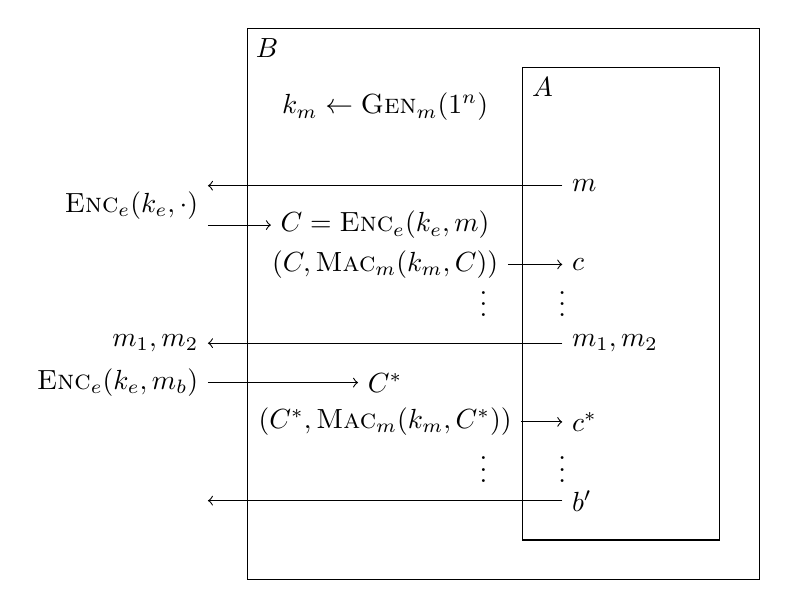
\begin{tikzpicture}
            \draw (1.5, -1) rectangle (8, 6);
            \draw (5, -0.5) rectangle (7.5, 5.5);
            \node at (1.75, 5.75) {$B$};
            \node at (5.25, 5.25) {$A$};

            \node at (3.25, 5) {$k_m \gets \textsc{Gen}_m(1^n)$};

            \node (enc) at (3.25, 3.5) {$C = \textsc{Enc}_e(k_e, m)$};
            \node (mac) at (3.25, 3) {$(C, \textsc{Mac}_m(k_m, C))$};

            \draw (5.5, 4) edge[->] node[right, pos=0] {$m$} (1, 4)
                (1, 3.5) edge[->] (enc)
                (mac) edge[->] node[right, pos=1] {$c$} (5.5, 3);
            \node[left] at (1, 3.75) {$\textsc{Enc}_e(k_e, \cdot)$};
            \node at (5.5, 2.6) {$\vdots$};
            \node at (4.5, 2.6) {$\vdots$};

            \draw (5.5, 2) edge[->] node[right, pos=0] {$m_1, m_2$} node[left, pos=1] {$m_1, m_2$} (1, 2);
            \node (enc-mb) at (3.25, 1.5) {$C^*$};
            \node (mac-mb) at (3.25, 1) {$(C^*, \textsc{Mac}_m(k_m, C^*))$};
            \draw (1, 1.5) edge[->] node[left, pos=0] {$\textsc{Enc}_e(k_e, m_b)$} (enc-mb);
            \draw (mac-mb) edge[->] node[right, pos=1] {$c^*$} (5.5, 1);

            \node at (5.5, 0.5) {$\vdots$};
            \node at (4.5, 0.5) {$\vdots$};

            \draw (5.5, 0) edge[->] node[right, pos=0] {$b'$} (1, 0);
        \end{tikzpicture}
    \end{center}

    To prove ciphertext integrity, suppose we have an adversary $A$ that breaks the ciphertext integrity of $\Pi$. Here, $A$ asks for ciphertext queries, and eventually returns a new ciphertext that is valid.

    We'd like to construct an adversary $B$ that is able to generate a new message and a tag, given oracle access to the MAC scheme. The construction will follow similarly to the prior proof on CPA security.

    Here, our adversary $B$ can sample $k_e \gets \mathsf{Gen}_e(1^n)$. When $A$ asks for the encryption of $M$, $B$ can send $m = \mathsf{Enc}_e(k_e, M)$ to the MAC oracle, and it returns $c = (m, t)$ to $A$.

    When $A$ returns $C^* = (c^*, t^*)$, $B$ can also just return the same, since the tag $t^*$ is being computed on $c^*$.

    \begin{center}
        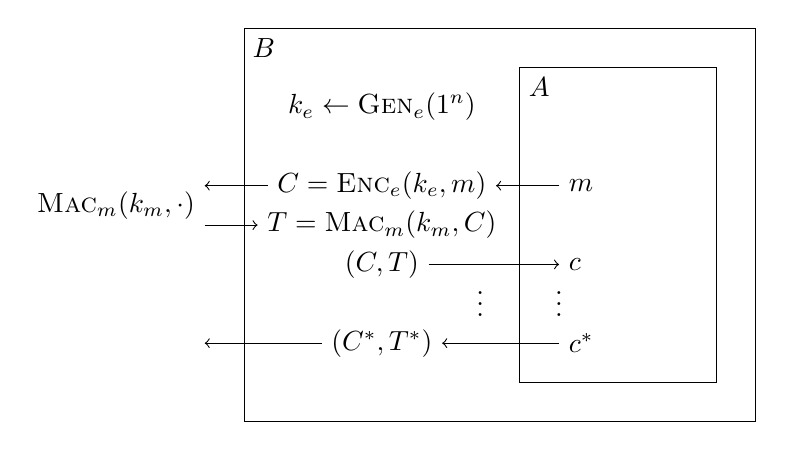
\begin{tikzpicture}
            \draw (1.5, 1) rectangle (8, 6);
            \draw (5, 1.5) rectangle (7.5, 5.5);
            \node at (1.75, 5.75) {$B$};
            \node at (5.25, 5.25) {$A$};

            \node at (3.25, 5) {$k_e \gets \textsc{Gen}_e(1^n)$};

            \node (enc) at (3.25, 4) {$C = \textsc{Enc}_e(k_e, m)$};
            \node (mac) at (3.25, 3.5) {$T = \textsc{Mac}_m(k_m, C)$};
            \node (enc-mac) at (3.25, 3) {$(C, T)$};

            \draw (5.5, 4) edge[->] node[right, pos=0] {$m$} (enc)
                (enc) edge[->] (1, 4)
                (1, 3.5) edge[->] (mac)
                (enc-mac) edge[->] node[right, pos=1] {$c$} (5.5, 3);
            \node[left] at (1, 3.75) {$\textsc{Mac}_m(k_m, \cdot)$};
            \node at (5.5, 2.6) {$\vdots$};
            \node at (4.5, 2.6) {$\vdots$};

            \node (gen-ciphertext) at (3.25, 2) {$(C^*, T^*)$};
            \draw (5.5, 2) edge[->] node[right, pos=0] {$c^*$} (gen-ciphertext)
                (gen-ciphertext) edge[->] (1, 2);
        \end{tikzpicture}
    \end{center}
\end{proof}

As an example, AES-GCM is the most popular authenticated encryption scheme that is used, and also has the ability to authenticate additional data. (AES-GCM basically just appends the associated data to the ciphertext, so that the encryption is only on the message, but the MAC is on both the ciphertext and the associated data.) This scheme uses a counter-mode encryption scheme, and the MAC that we saw, but makes this more efficient.

